\documentclass{article}
\usepackage{tikz, comment}
\usepackage{pifont}
\usepackage{fontspec, pgfplots}
\usetikzlibrary{arrows, decorations.markings, decorations.pathreplacing}
\begin{comment}
:Title: Not defined yet
:Tags: perimeter;end behavior;moment;pythagorean theorem;origin
:Prob: 0.5707;0.561;0.5416;0.5313;0.5306
:Author: Prof.Hu Ji-shan, HKUST
:Slug: No name yet

Description Here.........
\end{comment}
\begin{document}\centering 

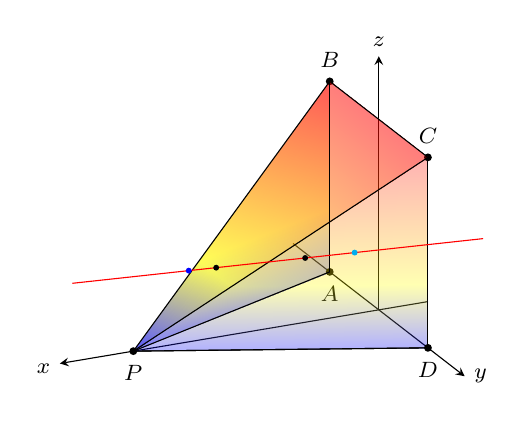
\begin{tikzpicture}[font=\footnotesize]
\pgfplotsset{compat=1.8}
\begin{axis}
[axis lines = center, view={155}{30}, scale=1, ticks=none,
axis background, xlabel = {$x$}, ylabel ={$y$}, zlabel ={$z$}, domain =-2:2, y domain =-2:2,
xmin =-200,
xmax =1299,
ymin =-699,
ymax =699,
zmin =0, 
zmax =799,
samples =10, samples y =40, z buffer = auto, 
every axis x label/.style={
    at={(ticklabel* cs:1)},
    anchor= east, yshift =-2
},
every axis y label/.style={
    at={(ticklabel* cs:1)},
    anchor= west,
},
every axis z label/.style={
    at={(ticklabel* cs:1)},
    anchor= south
}]

\addplot3[surf, shader=interp, mesh/cols=2, opacity=0.3] coordinates
		{(1000,0,0) (0,-400,0) (0,-400,600) (0,-400,600)};
\node[label={-90:{$P$}},circle,fill,inner sep=1pt] at (axis cs:1000,0,0) {};
\node[label={-90:{$A$}},circle,fill,inner sep=1pt] at (axis cs:0,-400,0) {};
\node[label={90:{$B$}},circle,fill,inner sep=1pt] at (axis cs:0,-400,600) {};

\addplot3[surf, shader=interp, mesh/cols=2, opacity=0.3] coordinates
		{(1000,0,0) (0,-400,600) (0,400,600) (0,400,600)};

\addplot3[surf, shader=interp, mesh/cols=2, opacity=0.3] coordinates
		{(1000,0,0) (0, 400,0) (0,400,600) (0,400,600)};
\node[label={90:{$C$}},circle,fill,inner sep=1pt] at (axis cs:0,400,600) {};
\node[label={-90:{$D$}},circle,fill,inner sep=1pt] at (axis cs:0,400,0) {};

\addplot3[surf, shader=interp, mesh/cols=2, opacity=0.3] coordinates
		{(1000,0,0) (0, -400,600) (0,400,600) (0,400,600)};

\addplot3[surf, black] coordinates
		{(1000,0,0) (0,-400,0) (0,-400,600)};
\addplot3[surf, black] coordinates
		{(1000,0,0) (0,-400,600)};

\addplot3[surf, black] coordinates
		{(1000,0,0) (0,400,600) (0,-400,600)};

\addplot3[surf, black] coordinates
		{(1000,0,0) (0,400,0) (0,400,600)};

\addplot3[surf, black] coordinates
		{(1000,0,0) (0,400,0) (0,400,600)};
		
\addplot3 [data cs=cart, red, domain=-200:1200, y domain = -1000:500] ({(8975 + 21*y)/13},{y},{(4775 + 9*y)*3/65});

\node[label={180:{}},circle,fill,inner sep=0.75pt] at (axis cs:125,-350,75) {};

\node[label={180:{}},circle, blue, fill,inner sep=0.75pt] at (axis cs:811.9,75.2,251.6) {};

\node[label={180:{}},circle, cyan, fill,inner sep=0.75pt] at (axis cs:-166.7, -530.6, 0) {};

\node[label={180:{}},circle,fill,inner sep=0.75pt] at (axis cs:650,-25,210) {};

\end{axis}

\end{tikzpicture}\hskip 1cm
\end{document}